\documentclass{article}
\usepackage[utf8x]{inputenc}
\usepackage{ucs}
\usepackage[russian]{babel}
\usepackage{graphicx}
\usepackage[unicode]{hyperref}
\usepackage{tabularx}
\usepackage{color}
\usepackage{index}
\hypersetup{
  bookmarks=true,
  colorlinks=false,
  unicode=true
}

%----------------------------------------------------------------------------------
\title{Фильтрация наблюдений угловых скоростей и ориентации колесного робота}
\author{Кирилл Андреев}

%----------------------------------------------------------------------------------
\begin {document}
%----------------------------------------------------------------------------------
\maketitle
%----------------------------------------------------------------------------------
\begin {abstract}
В документе представлено описание алгоритмов обработки данных гироскопа и
магнитометра для определения ориентации колесного робота в общем случае
(определение углов крена, тангажа и рысканья).
\end{abstract}
\tableofcontents
\pagebreak
%----------------------------------------------------------------------------------
\section{Введение}
%----------------------------------------------------------------------------------
Гироскоп позволяет определить компоненты угловой скорости тела в
\emph{инерциальных} осях. Однако, поскольку начальное положение гироскопа не
может быть измерено точно, гироскопу свойственны смещения в показаниях
значений угловой скорости. Вторым важным параметром гироскопа является его
стабильность, характеризуемая средним значением ошибки, которая накапливается
за единицу времени. Для исследования параметров стабильности используется
дисперсия Аллана~\cite{vectorNav}.
%----------------------------------------------------------------------------------
\section{Описание вращений твердого тела}
%----------------------------------------------------------------------------------
Решение задачи нахождения ориентации твердого тела по наблюдениям угловых
скоростей требуют написания уравнений вращательной динамики твердого тела. Для
описания вращения твердого тела воспользуемся кватернионами. Представление
поворотов твердого тела с помощью кватернионов имеет ряд преимуществ
\cite{amelkinMIPT}:
\begin{itemize}
\item отсутствие вырождений, присущих углам Эйлера,
\item простые уравнения динамики,
\item уравнения динамики представлены небольшим числом параметров.
\end{itemize}
%----------------------------------------------------------------------------------
\subsection{Алгебра кватернионов}
%----------------------------------------------------------------------------------
Кватернион представляет собой четырехмерное гиперкомплексное число и
записывается в виде
$$
\mathbf{\Lambda} = \lambda_0 \mathbf{i}_0 + \lambda_1 \mathbf{i}_1 + \lambda_2
\mathbf{i}_2 + \lambda_3 \mathbf{i}_3 = \lambda_0 + \mathbf{\lambda},
$$
где форма $\lambda_0 + \mathbf{\lambda}$ представляет собой разложение в виде
скалярной и векторной частей.

Правила умножения для кватернионов можно записать с помощью правила умножения
базисных векторов:
$$
\mathbf{i}_k\circ\mathbf{i}_j = -\left(\mathbf{i}_k \cdot\mathbf{i}_j\right) +
\mathbf{i}_k\times\mathbf{i}_j.
$$
Формула для произведения кватернионов имеет следующий вид:
$$
\mathbf{\Lambda}\circ\mathbf{M} = \left(\lambda_0
+\mathbf{\lambda}\right)\circ\left(\mu_0 + \mathbf{\mu}\right) = 
\lambda_0\mu_0 -\left(\mathbf{\lambda}\cdot\mathbf{\mu}\right) +
\lambda_0\mathbf{\mu} + \mu_0\mathbf{\lambda} +
    \mathbf{\lambda}\times\mathbf{\mu}.
$$
Свойства умножения кватернионов:
\begin{enumerate}
\item Умножение кватернионов обладает дистрибутивными по отношению к сложению
    свойствами (сложение представляет собой покомпонентное сложение)
$$
\mathbf{\Lambda}\circ\left(\mathbf{M} + \mathbf{N}\right) =
\mathbf{\Lambda}\circ\mathbf{M} +
\mathbf{\Lambda}\circ\mathbf{N}
$$
\item Умножение кватернионов ассоциативно, т. е
$$
\mathbf{\Lambda}\circ\mathbf{M}\circ\mathbf{N} = 
\mathbf{\Lambda}\circ\left(\mathbf{M}\circ\mathbf{N}\right) = 
\left(\mathbf{\Lambda}\circ\mathbf{M}\right)\circ\mathbf{N} 
$$
\item Кватернионное умножение не обладает свойствами коммутативности, т. е.
$$
\mathbf{\Lambda}\circ\mathbf{M}\not\equiv\mathbf{M}\circ\mathbf{\Lambda}
$$
\item Скалярная часть кватерниона не изменяется при циклической перестановке
сомножителей, т. е. 
$$
scal\left(\mathbf{\Lambda}\circ\mathbf{M}\circ\mathbf{N}\right) =
scal\left(\mathbf{N}\circ\mathbf{\Lambda}\circ\mathbf{M}\right)
$$
\end{enumerate}

Обратный кватернион определяется таким образом, что
$$
\mathbf{\Lambda}\circ\mathbf{\Lambda}^{-1} = 1.
$$

Сопряженный кватернион и норма кватерниона вводится по аналогии с комплексными
числами. Нормированный или единичный кватернион имеет единичную норму.

Пусть $\mathbf{\Lambda}$ -- нормированный кватернион. Тогда его можно
представить в тригонометрической форме: $\lambda_0 = \cos{\nu},
\mathbf{\lambda} = \mathbf{e}\sin{\nu}$, где $\mathbf{e}$ -- единичный вектор,
коллинеарный $\mathbf{\lambda}$. Умножение кватернионов с коллинеарными
векторными частями в тригонометрической
форме аналогично форме Муавра для умножения комплексных чисел. Пусть
$\mathbf{\Lambda}_1 = \left|\mathbf{\Lambda}_1\right|\left(\cos{\phi_1}
+\mathbf{e}\sin{\phi_1}\right)$, $\mathbf{\Lambda}_2 =
\left|\mathbf{\Lambda_2}\right|\left(\cos{\phi_2}
+\mathbf{e}\sin{\phi_2}\right)$, тогда
$$
\mathbf{\Lambda}_1\circ\mathbf{\Lambda}_2 =
\left|\mathbf{\Lambda_1}\right|\left|\mathbf{\Lambda_2}\right|\left(\cos{\left(\phi_1+\phi_2\right)}+\mathbf{e}\sin{\left(\phi_1+\phi_2\right)}\right)
$$
%----------------------------------------------------------------------------------
\subsection{Повороты твердого тела}
%----------------------------------------------------------------------------------
\begin{figure}
\centering
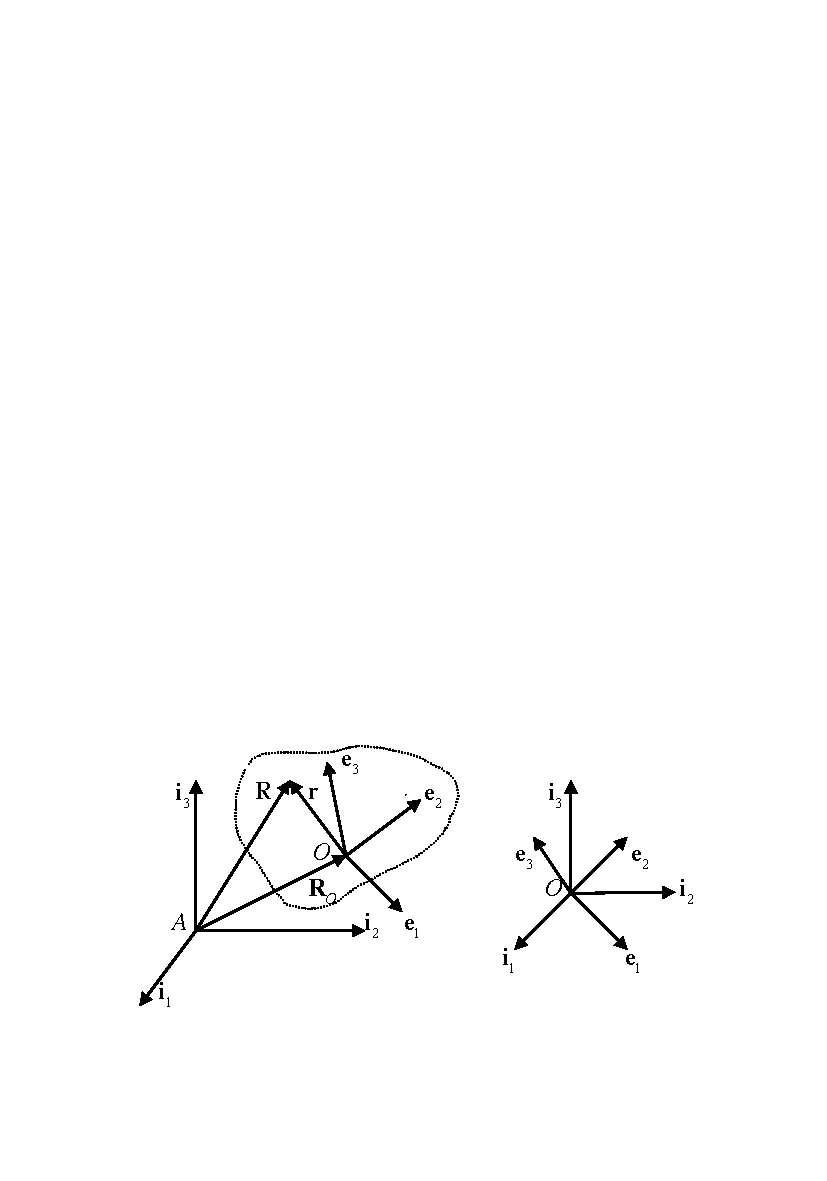
\includegraphics[width=0.8\textwidth]{pic/BI_notations.pdf}
\caption{\label{fig:BI_notation}Обозначения инерциальной системы отсчета
$A\mathbf{i}_1\mathbf{i}_2\mathbf{i}_3$ и системы
$O\mathbf{e}_1\mathbf{e}_2\mathbf{e}_3$ собственных осей твердого тела, в
котором координаты каждой точки твердого тела неизменны.}
\end{figure}
Твердое тело обладает свойством сохранения координат точек в некотором
локальном правом (или левом) ортонормированном базисе
$O\mathbf{e}_1\mathbf{e}_2\mathbf{e}_3$, связанным с твердым телом. Для того,
чтобы знать координаты всех точек твердого тела в системе отсчета
$O\mathbf{e}_1\mathbf{e}_2\mathbf{e}_3$, необходимо знать положение базиса
$O\mathbf{e}_1\mathbf{e}_2\mathbf{e}_3$ относительно базиса
$A\mathbf{i}_1\mathbf{i}_2\mathbf{i}_3$.
$$
\mathbf{R}=\mathbf{R}_0+\mathbf{r} = \mathbf{R}_0 +
\sum_{k=1}^{3}r_k\mathbf{e}_k.
$$
Движение точки $O$ представляет собой поступательное движение твердого тела,
движение базиса $O\mathbf{e}_1\mathbf{e}_2\mathbf{e}_3$ относительно базиса
$O\mathbf{i}_1\mathbf{i}_2\mathbf{i}_3$ представляет собой вращение твердого
тела.
%----------------------------------------------------------------------------------
\subsection{Кватернионное представление вращений}
%----------------------------------------------------------------------------------
Вращение твердого тела с неподвижной точкой задается нормированным
кватернионом $\mathbf{\Lambda}$ по формулам
$$
\mathbf{e}_k =
\mathbf{\Lambda}\circ\mathbf{i}_k\circ\overline{\mathbf{\Lambda}},
$$
при этом каждому положению тела соответствуют два кватерниона, отличающихся
знаком.

Получим выражение для искомого кватерниона в явном виде. Для этого введем
обозначения
$$
\mathbf{r}_k = \mathbf{e}_k - \mathbf{i}_k,\quad \mathbf{s}_k = \mathbf{e}_k +
\mathbf{i}_k ;\quad k=1, 2, 3.
$$
Для этих векторов выполнены следующие соотношения:
$$
\mathbf{s}_k\cdot\mathbf{r}_k = 0, \quad \mathbf{s}_j\cdot\mathbf{r}_k =
-\mathbf{s}_k\cdot\mathbf{r}_j
$$
Запишем теперь уравнения для искомого кватерниона в следующем виде (домножив
исходные уравнения на кватернион $\mathbf{\Lambda}$ справа:
$$
\mathbf{e}_k\circ\mathbf{\Lambda} = \mathbf{\Lambda}\circ\mathbf{i}_k,
$$
что можно переписать в виде следующей системы:
$$
\left\{
\begin{array}{l}
    \mathbf{e}_k\mathbf{\lambda} = \mathbf{i}_k\mathbf{\lambda} \\
    \lambda_0\mathbf{e}_k + \mathbf{e}_k\times\mathbf{\lambda} =
    \lambda_0\mathbf{i}_k - \mathbf{i}_k\times\mathbf{\lambda}
\end{array}
\right. \Rightarrow
\left\{
\begin{array}{l}
    \mathbf{r}_k\cdot\mathbf{\lambda} = 0 \\
    \lambda_0\mathbf{r_k} = \mathbf{\lambda}\times\mathbf{s}_k
\end{array}
\right. .
$$
В случае, если базисы совпадают, решение $\lambda_0=\pm 1$ очевидно. Пусть в
общем случае векторы $\mathbf{r}_1$ и $\mathbf{r}_2$ не равны нулю. Тогда
векторная часть искомого решения может быть записана в виде $\mathbf{\lambda}
= x\left(\mathbf{r}_1\times\mathbf{r}_2\right)$, где $x$ -- некоторый скаляр.
Подставляя полученное выражение во второе уравнение системы, получаем, что
$$
\left\{
\begin{array}{l}
    \lambda_0\mathbf{r}_1 =
    -x\mathbf{s}_1\times\left(\mathbf{r}_1\times\mathbf{r}_2\right)
    =-x\mathbf{r}_1\left(\mathbf{s}_1\cdot\mathbf{r}_2\right)\\
    \lambda_0\mathbf{r}_2 =
    -x\mathbf{s}_2\times\left(\mathbf{r}_1\times\mathbf{r}_2\right)
    =-x\mathbf{r}_2\left(\mathbf{s}_2\cdot\mathbf{r}_1\right)\\
\end{array}
\right. .
$$
Оба полученных уравнение тождественно равны, потому
$$
\mathbf{\Lambda} = x\left(\mathbf{s}_2\cdot\mathbf{r}_1 +
\mathbf{r}_1\times\mathbf{r}_2\right)
$$

Теорема Эйлера о вращении твердого тела следует непосредственно из приведения
кватерниона к тригонометрическому виду
$\mathbf{\Lambda}=\left(\cos{\phi}+\mathbf{e}\sin{\phi}\right)$:
\begin{itemize}
\item Вращение тела осуществляется вдоль оси, направление которой совпадает с
    векторной частью кватерниона
\item Угол поворота составляет $2\phi$.
\end{itemize}
Кватернионное сложение поворотов представляет собой умножение кватернионов
(см.~рис.~\ref{fig:quat_multiply}). Пусть $\mathbf{\Lambda}$ задает поворот из
базиса $\mathbf{I}$ в базис $\mathbf{I}'$, а кватернион $\mathbf{M}$ -- из
базиса $\mathbf{I}'$ в базис $\mathbf{I}''$. Тогда начальное положение точки
$\mathbf{r}$ преобразуется в конечное положение точки $\mathbf{r}''$ в соответствии с
преобразованием
$$
\mathbf{r}'' = \mathbf{M}\circ\mathbf{r}'\circ\overline{\mathbf{M}} =
\mathbf{M}\circ\mathbf{\Lambda}\circ\mathbf{r}\circ\overline{\mathbf{\Lambda}}\circ\overline{\mathbf{M}}
= \mathbf{N}\circ\mathbf{r}\circ\overline{\mathbf{N}}, \quad \mathbf{N} =
\mathbf{M}\circ\mathbf{\Lambda}
$$
\begin{figure}
\centering
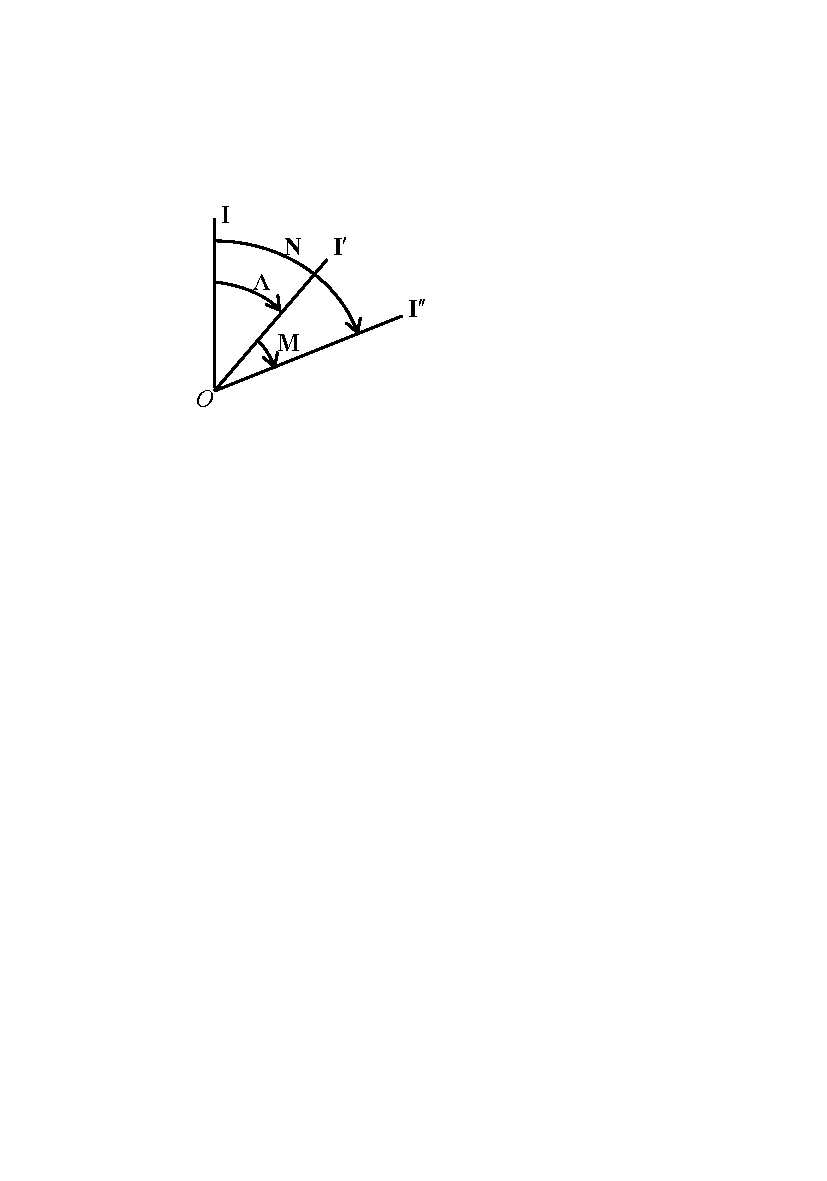
\includegraphics[width=0.4\textwidth]{pic/multiple_rotations.pdf}
\caption{\label{fig:quat_multiply}Сложение поворотов c помощью перемножения
кватернионов}
\end{figure}

Для написания уравнений движения твердого тела и дальнейшей фильтрации
наблюдений необходимо записать уравнение производной для кватерниона, а затем
эти уравнения линеаризовать. Динамика кватерниона задается уравнением
Пуассона, которое выводится следующим образом.

В соответствии с определением, угловой скоростью (вектор в базисе
$\mathbf{I}$) является следующая величина
$$
\mathbf{\omega}=\lim_{\Delta t \rightarrow 0}\frac{\Delta\phi\left(t,\Delta t\right)}{\Delta
t}\mathbf{e}\left(t,\Delta t\right)
$$
Изменению поворота соответствует следующее изменение кватерниона
$$
\delta\mathbf{\Lambda}=\cos{\frac{\Delta\phi\left(t,\Delta t\right)}{2}} + \mathbf{e}\left(t,\Delta t\right)
\sin{\frac{\Delta\phi\left(t,\Delta t\right)}{2}} = 1 + \mathbf{e}\left(t,\Delta t\right)
{\frac{\Delta\phi\left(t,\Delta t\right)}{2}} + O\left(\left(\Delta\phi\right)^2\right)
$$
Этот кватернион определяется из формулы сложения поворотов:
$$
\mathbf{\Lambda}\left(t+\Delta t\right) = \delta \mathbf{\Lambda} \circ
\mathbf{\Lambda}\left(t\right)
$$
$$
\mathbf{\Lambda}\left(t+\Delta t\right) - \mathbf{\Lambda}\left(t\right)
=\delta \mathbf{\Lambda}\circ\mathbf{\Lambda}\left(t\right)
-\mathbf{\Lambda}\left(t\right) \Rightarrow \Delta \mathbf{\Lambda} =
\left(\delta \mathbf{\Lambda}-1\right)\circ \mathbf{\Lambda}\left(t\right)
$$
Вычисляя предел при $\Delta t \rightarrow 0$, получаем следующие соотношения:
$$
\dot{\mathbf{\Lambda}} = \lim_{\Delta t \rightarrow 0}{\frac{\Delta
\mathbf{\Lambda}}{\Delta t}} =  \lim_{\Delta t \rightarrow 0}{\frac{\delta
\mathbf{\Lambda}}{\Delta t}}\circ \mathbf{\Lambda}\left( t \right) =
\frac{1}{2}\mathbf{\omega}_I\circ\mathbf{\Lambda}.
$$
Полученные уравнения являются являются кинематическими уравнениями
вращательного движения твердого тела, записанными в кватернионах, и называются
уравнениями Пуассона -- четыре скалярных дифференциальных уравнения, которые
связывают параметры Родрига-Гамильтона с проекциями угловой скорости тела
на оси базиса $\mathbf{I}$ -- инерциальной системы отсчета.

В некоторых ситуациях угловая скорость задается в проекциях на оси базиса,
связанного с телом. В этом случае
$$
\mathbf{\omega}_I =
\mathbf{\Lambda}\circ\mathbf{\omega}_B\circ\overline{\mathbf{\Lambda}}.
$$
Тогда уравнение Пуассона имеет иной вид:
$$
\dot{\mathbf{\Lambda}} = \frac{1}{2}\mathbf{\Lambda}\circ\mathbf{\omega}_B.
$$
Полученное уравнение будет использоваться при составлении уравнений фильтра
для показаний датчика угловых скоростей (ДУС).
%----------------------------------------------------------------------------------
\section{Линеаризация вращений твердого тела и расширенный фильтр Калмана}
%----------------------------------------------------------------------------------
При решении задачи нахождения ориентации твердого тела в качестве фазовых
переменных рассмотрим следующие:
\begin{itemize}
\item[$q_{BI}$] кватернион, задающий ориентацию тела -- векторная его часть,
    скалярная может быть вычислена исходя из единичной нормы кватерниона;
\item[$\omega_B$] вектор угловой скорости, заданный в проекциях на \emph{собственные
    оси} твердого тела.
\item[$\omega_{I}^{bias}$] смещение показаний гироскопа, выраженное в
    проекциях на \emph{инерциальные} оси.
\end{itemize}
Удобство использования оценки угловой скорости, выраженной в проекциях на
собственные оси, состоит в следующем:
\begin{enumerate}
    \item Оценка угла поворота колес задает соответствие между линейной
        скоростью движения и угловой скоростью в собственных осях
    \item Разность ускорений, измеренных в точке центра масс и в любой другой
        точке твердого тела, определяется из соотношения угловых скоростей,
        выраженных в собственных осях и геометрией расположения
        акселерометров.
\end{enumerate}

Наличие смещения в показаниях гироскопа (или датчика угловых скоростей -- ДУС)
вызвано как минимум тем, что начальное положение тела не может быть известно
точно. Таким образом, оценка скорости вращения $\hat{\omega}_B$ содержит в
себе смещение показаний ДУС.

В связи с наличием смещений оценить положение тела только по показаниям
гироскопа не представляется возможным. В связи с этим в задаче рассмотрен
случай, когда в качестве дополнительного канала измерений имеется некоторое
направление, задаваемое некоторым вектором, истинное значение которого
известно заранее. Примером такого направления может послужить вектор
напряженности магнитного поля Земли или направление силы тяжести.

Далее при реализации фильтра Калмана будет рассмотрена задача наблюдений таких
опорных векторов. Для решения задачи необходимо привести систему уравнений,
описывающих динамику твердого тела и наблюдений к линейному виду.
%----------------------------------------------------------------------------------
\subsection{Линеаризация динамики твердого тела}
%----------------------------------------------------------------------------------
Для начала перепишем уравнение Пуассона в матричном виде, обозначив отдельно
скалярную и векторную части кватерниона
$$
\left(
\begin{array}{c}
    \dot{q}_0 \\
    \dot{\mathbf{q}}
\end{array}
\right) = \frac{1}{2}\mathbf{C}
\left(
\begin{array}{c}
    {q}_0 \\
    {\mathbf{q}}
\end{array}
\right),
\quad
\mathbf{C} = \left(\begin{array}{cc}
0 & -\mathbf{\omega}^T \\
\mathbf{\omega} & \mathbf{W} 
\end{array}\right), \quad
\mathbf{W} = \left(\begin{array}{rrr}
        0 & \omega_3 & -\omega_2 \\
        -\omega_3 & 0 & \omega_1 \\
        \omega_2 & -\omega_1 & 0
\end{array}\right)
$$

На шаге экстраполяции фильтра Калмана приращение к оценке состояния
$\delta\hat{\rho}_{t_{k+1}|t_k}$ задается выражением
$$
\delta\hat{\rho} = \mathbf{F}\hat{\rho}\Delta t,
$$
где $\mathbf{F}$ представляет собой линеаризованную динамику состояния
$$
\delta\dot{\rho} = \mathbf{F}\delta\rho.
$$
В рассматриваемой задаче
$$
\rho = \left(\mathbf{q}_{BI}, \mathbf{\omega}_B,
\mathbf{\omega}_I^{bias}\right),
$$
причем в фазовый вектор включена только векторная часть кватерниона, поскольку
норма кватерниона, задающего ориентацию твердого тела, равна единице.В данном
уравнении в качестве приращения кватерниона будем считать приращение поворота
тела, то есть
$$
\hat{q}_{k+1} = \delta q \circ \hat{q}_{k},
$$
причем дальнейшая линеаризация зависит от порядка перемножения кватернионов.
Линеаризуя уравнение Пуассона с учетом того, что оценка угловой скорости в
собственных координатах включает в себя смещение ДУС, записанное в
инерциальных координатах, получаем, что первые три ряда матрицы $\mathbf{F}$
имеют вид
$$
\left(\begin{array}{ccc}
        \mathbf{0}_{3\times 3} & \frac{1}{2}\mathbf{A}^T &
        -\frac{1}{2}\mathbf{E}_{3\times 3}
\end{array}\right),
$$
остальные элементы матрицы равны нулю.  Матрица $\mathbf{A}$ задает следующее
линейное  преобразование:
$$
\mathbf{\omega}_B = \mathbf{A}\mathbf{\omega}_I, 
$$
$\mathbf{0}_{3\times 3}$ и $\mathbf{E}_{3\times 3}$ -- нулевая и единичная
матрицы размером $3\times 3$. Такая динамика соответствует модели движения,
при которой изменение угловой скорости и смещения ДУС представляют собой белый
шум.

Для валидации полученной модели движения проведем следующий вычислительный
эксперимент. Сначала задается некоторые случайные значения $q_{BI}$, $\omega_B$ и
$\omega_I^{bias}$, после чего запускается фильтр Калмана с начальной оценкой
фазового вектора, соответствующей выбранным параметрам. Далее, используя
только шаг предиктора, строится фазовая траектория кватерниона. Затем эта же
фазовая траектория кватерниона строится на основании решения уравнения
Пуассона. В случае, если линеаризация осуществлена верно, при уменьшении шага
времени $\Delta t$, ошибка между точной и линеаризованной траекториями должна
уменьшаться. Результаты представлены на рисунках
\ref{fig:kalman_predictor_val_e-1} -- \ref{fig:kalman_predictor_val_e-3}.
Стоит отметить, что при $\omega_I^{bias} = 0$ и при $\Delta t = 10^{-1}$ сек
точность линейной экстраполяции остается приемлемой на протяжении около 5
минут.
\begin{figure}
\centering
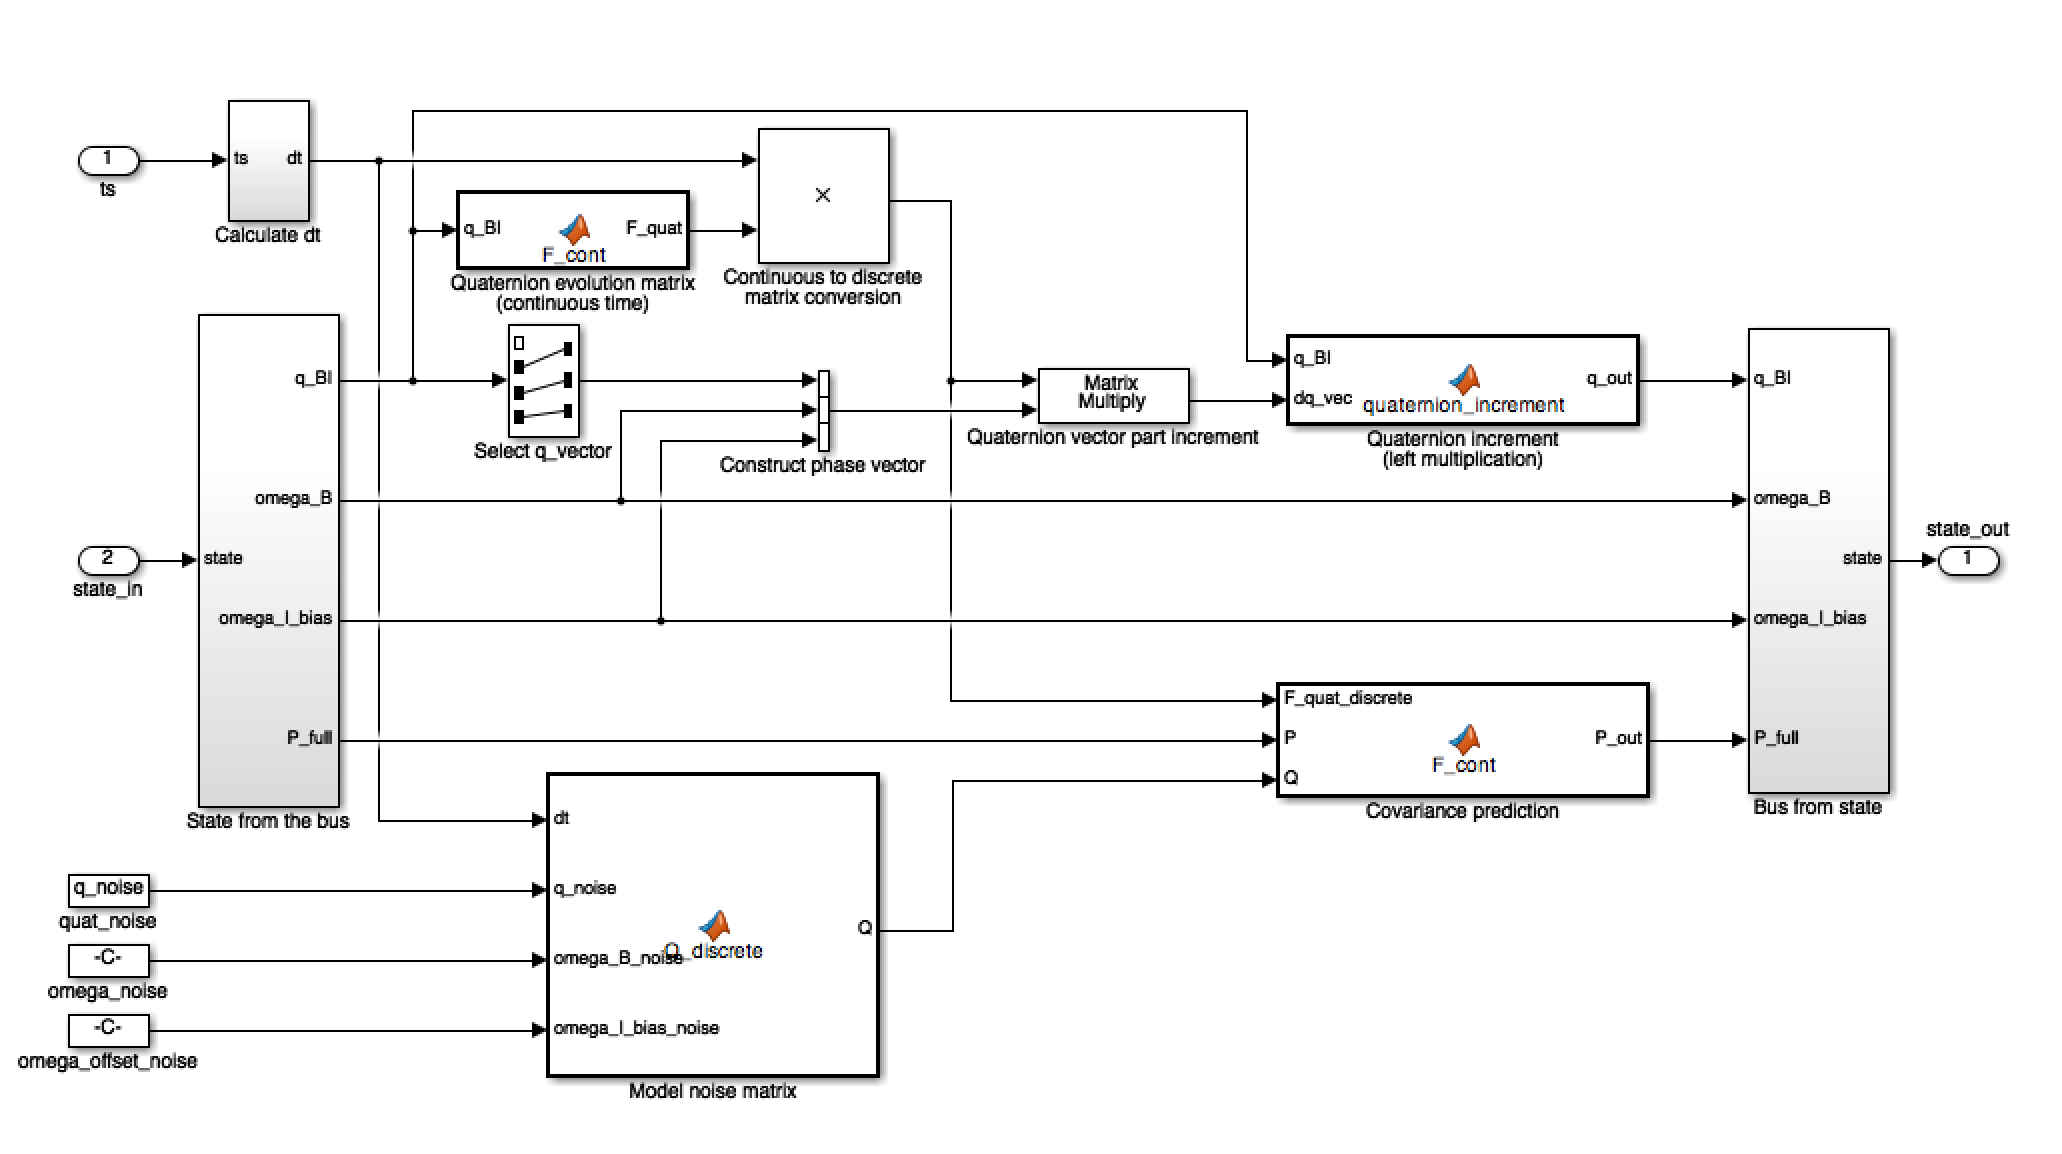
\includegraphics[width=0.8\textwidth]{pic/kalman_predictor.png}
\caption{\label{fig:kalman_predictor}Simulink-модель предиктора фильтра
Калмана}
\end{figure}
\begin{figure}
\centering
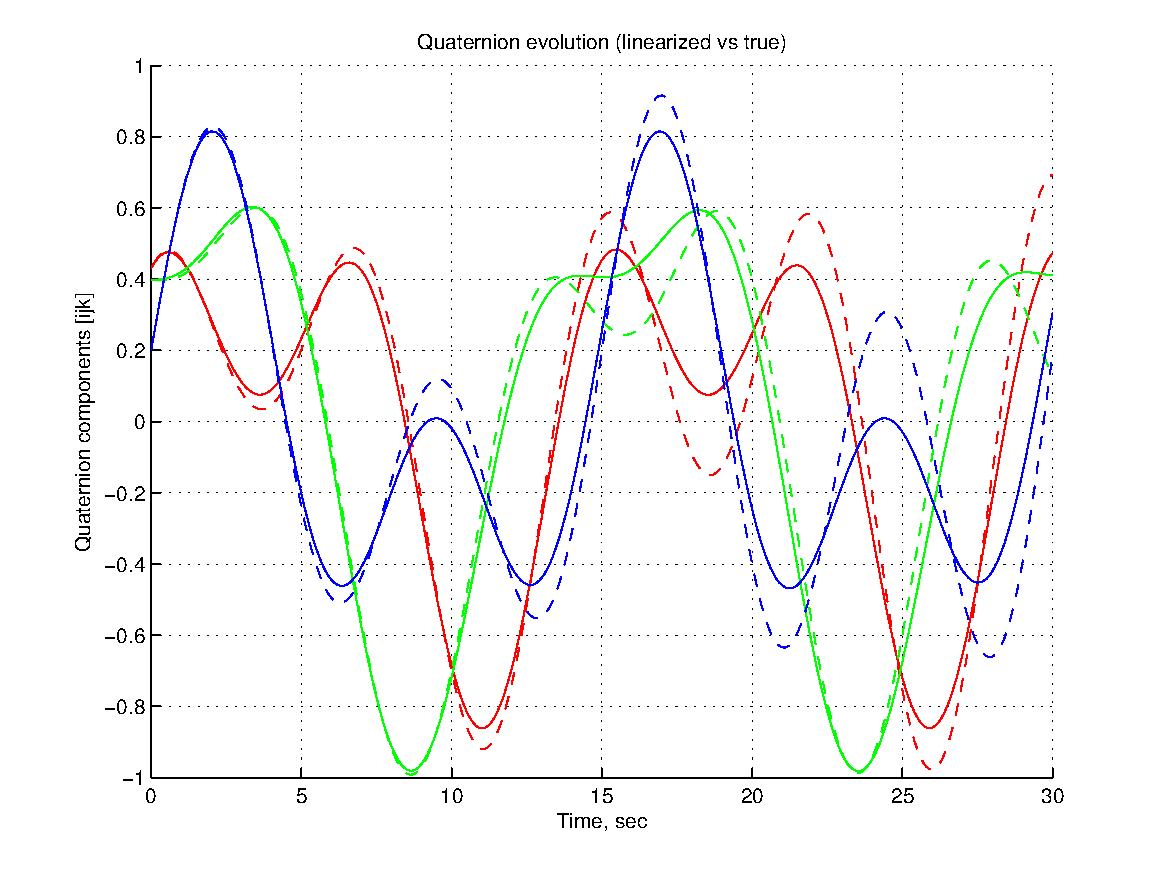
\includegraphics[width=0.8\textwidth]{pic/extrapolation_01.pdf}
\caption{\label{fig:kalman_predictor_val_e-1}Фазовые траектории векторной
    части кватерниона при
$\Delta t = 10^{-1}$ с}
\end{figure}
\begin{figure}
\centering
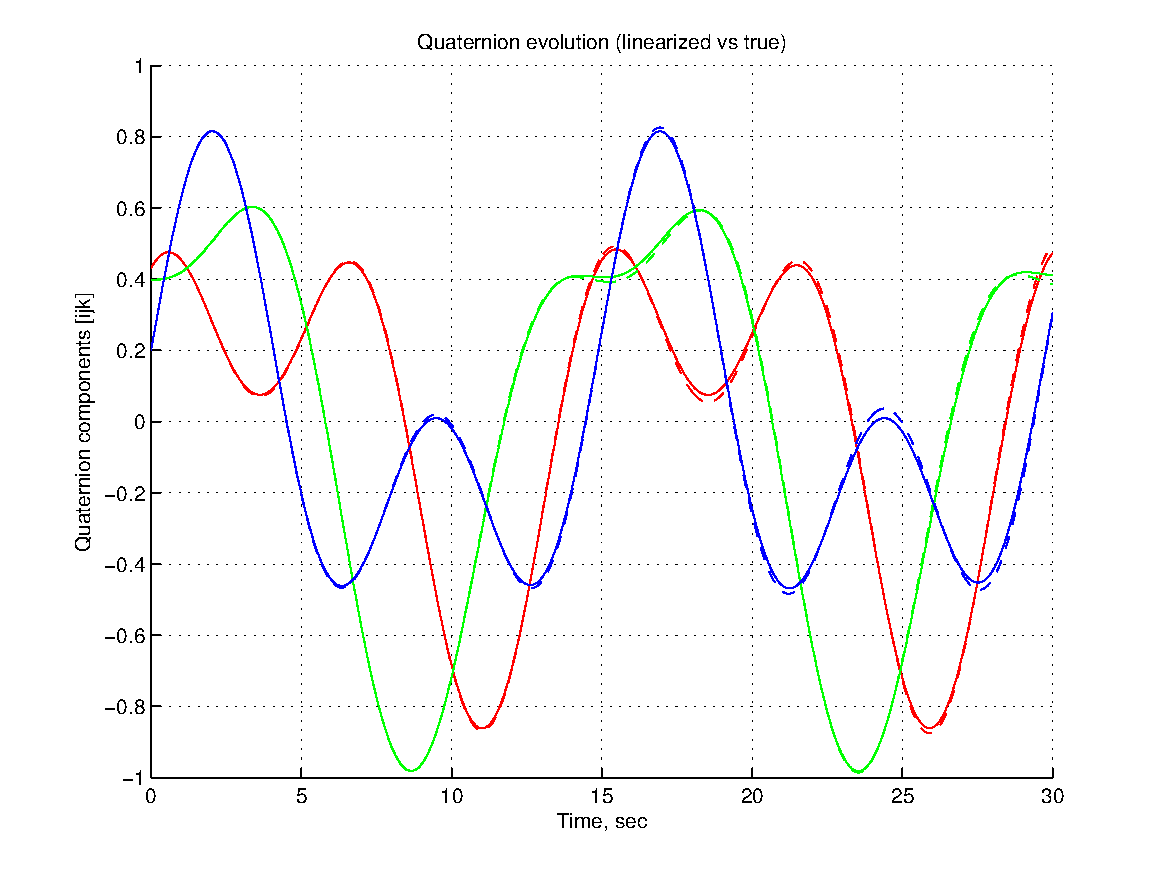
\includegraphics[width=0.8\textwidth]{pic/extrapolation_001.pdf}
\caption{\label{fig:kalman_predictor_val_e-2}Фазовые траектории векторной
    части кватерниона при
$\Delta t = 10^{-2}$ с}
\end{figure}
\begin{figure}
\centering
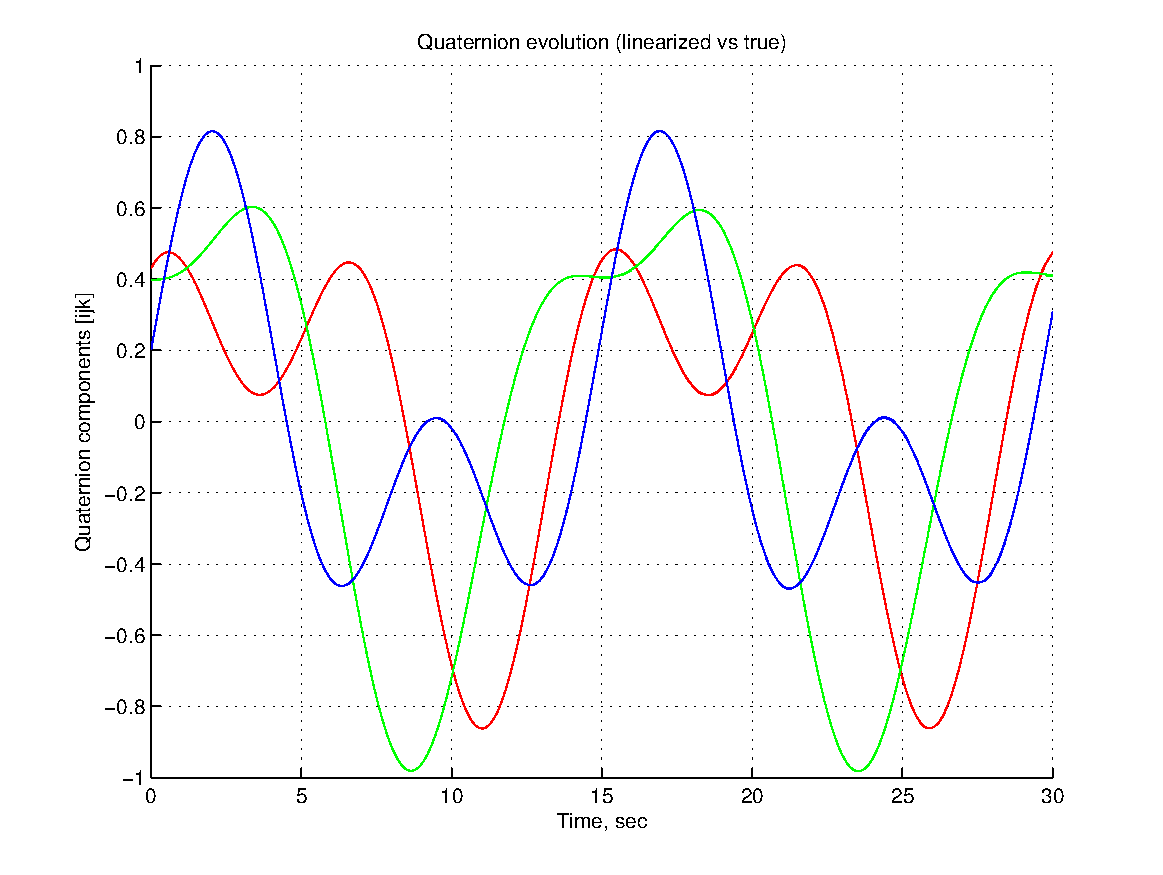
\includegraphics[width=0.8\textwidth]{pic/extrapolation_0001.pdf}
\caption{\label{fig:kalman_predictor_val_e-3}Фазовые траектории векторной
    части кватерниона при
$\Delta t = 10^{-3}$ с}
\end{figure}
Для воспроизведения полученных результатов необходимо запустить скрипт
$testLinearExtrapolation$ модели, предварительно выполнив скрипт $startup.m$.
%----------------------------------------------------------------------------------
\subsection{Линеаризация наблюдений}
%----------------------------------------------------------------------------------
Линейная функция наблюдений имеет следующий вид:
$$
z = \mathbf{H}\rho \quad \Rightarrow \quad \delta z = \mathbf{H} \delta \rho
$$
\subsubsection{Показания гироскопа}
Показания гироскопа представляют собой оценку угловой скорости вращения тела,
выраженную в проекциях на инерциальные оси. Кроме того, у данных показаний
имеется смещение, которое также выражено в инерциальных осях. Ожидаемое
значение этого наблюдения
$$
\hat{\mathbf{\omega}}_{meas} = \mathbf{A}^T\hat{\mathbf{\omega}_B},
$$
где матрица $ \mathbf{A}$ задает преобразование $\mathbf{\omega}_B =
\mathbf{A}\mathbf{\omega}_I$. Истинное наблюдение представляет собой ожидаемое
наблюдение с некоторым (малым) возмущением)
$$
\mathbf{\omega}_m = \hat{\mathbf{\omega}} + \delta\mathbf{\omega}
$$
С учетом того, что
$$
\mathbf{A}\left(\delta q \circ q\right) =
\mathbf{A}\left(\delta q\right)\mathbf{A}\left(q\right),
$$
а матрица поворота, определяемая малым кватернионом (т. е. кватернионом с
малой векторной частью), имеет вид
$$
\mathbf{A}\left(\delta q\right) = \mathbf{E} + 2\mathbf{W}_{\delta q},\quad
\mathbf{A}^T\left(\delta q\right) = \mathbf{E} - 2\mathbf{W}_{\delta q},
$$
где $\mathbf{W}_{\delta q}$ -- матрица косо-симметричного оператора, взятого со
знаком минус (аналогично $\mathbf{W}$). Тогда легко получить, что 
$$
\hat{\mathbf{\omega}}_m +\delta \mathbf{\omega}_m = \mathbf{A}^T\left(\delta q \circ
\hat{q}\right)\left(\hat{\mathbf{\omega}}_B + \delta \mathbf{\omega}_B\right) = 
\left(\mathbf{E} - 2\mathbf{W}_{\delta q}\right)\mathbf{A}^T\left(\hat{q}\right)
\left(\hat{\mathbf{\omega}}_B + \delta\mathbf{\omega}_B\right),
$$
$$
\hat{\mathbf{\omega}}_m +\delta \mathbf{\omega}_m = 
-2\mathbf{W}_{\delta q}\mathbf{A}^T\left(\hat{q}\right)\hat{\mathbf{\omega}}_B + 
\mathbf{A}^T\left(\hat{q}\right)
\left(\hat{\mathbf{\omega}}_B + \delta\mathbf{\omega}_B\right),
$$
$$
\delta \mathbf{\omega}_m = 
-2\mathbf{W}_{\delta q}\mathbf{A}^T\left(\hat{q}\right)\hat{\mathbf{\omega}}_B + 
\mathbf{A}^T\left(\hat{q}\right)\delta\mathbf{\omega}_B = 
-2\mathbf{W}_{\delta q}\hat{\mathbf{\omega}}_I + 
\mathbf{A}^T\left(\hat{q}\right)\delta\mathbf{\omega}_B.
$$
Окончательно (с учетом свойств антикоммутативности векторного произведения)
$$
\delta \mathbf{\omega}_m = 2\mathbf{W}_{\hat{\mathbf{\omega}}_I} \delta q+ 
\mathbf{A}^T\left(\hat{q}\right)\delta\mathbf{\omega}_B.
$$
Таким образом, матрица наблюдения показаний гироскопа имеет следующий вид
$$
\mathbf{H} = \left(\begin{array}{ccc}
2\mathbf{W}_{\hat{\mathbf{\omega}}_I} &
\mathbf{A}^T\left(\hat{q}\right) &
\mathbf{0}_{3\times 3}
\end{array}\right)
$$
Для валидации полученной линеаризованной зависимости выбираются случайные
величины $\hat{q}$, $\hat{\mathbf{\omega}}_B$, и некоторые малые возмущения
$\delta q$ и $\delta\mathbf{\omega}_B$. В приведенных ниже результатах теста
компоненты опорных значений выбирались из стандартного нормального
распределения, а возмущений -- из нормального распределения со средним $0$ и
дисперсией $\frac{1}{n}$. Запуская несколько независимых испытаний,
вычисляется среднее отношение ошибки между точным значением вариации $\delta
\rho$ и линеаризованным к величине возмущения. Для различных значений $n$
проверяется, что это отношение равно $O\left(\frac{1}{n}\right)$.
%----------------------------------------------------------------------------------
\subsubsection{Опорное направление}
%----------------------------------------------------------------------------------
Пусть в инерциальной системе отсчета имеется некоторое опорное направление,
задаваемое вектором $r_I$. Сенсоры на борту робота позволяют измерить
компоненты этого вектора в собственных осях, то есть компоненты вектора $r_B$.
$$
\mathbf{r}_m = \hat\mathbf{{r}}_B + \delta \mathbf{r} = \mathbf{A}\left(\delta
q\circ \hat{q}\right)\left(\hat{\mathbf{r}}_I + \delta \mathbf{r}_I\right) = 
\mathbf{A}\left(\hat{q}\right)
\left(\mathbf{E} + 2\mathbf{W}_{\delta q}\right)\left(\hat{\mathbf{r}}_I +
\delta \mathbf{r}_I\right),
$$

$$
\delta \mathbf{r} =
2\mathbf{A}\left(\hat{q}\right)\mathbf{W}_{\delta q}\hat{\mathbf{r}}_I = 
-2\mathbf{A}\left(\hat{q}\right)\mathbf{W}_{\hat{\mathbf{r}}_I}\delta q.
$$
Таким образом, матрица наблюдений опорного направления имеет вид
$$
\mathbf{H} = \left(\begin{array}{ccc}
-2\mathbf{A}\left(\hat{q}\right)\mathbf{W}_{\hat{\mathbf{r}}_I} &
\mathbf{0}_{3\times 3} &
\mathbf{0}_{3\times 3}
\end{array}\right)
$$
и имеет ранг 2. Таким образом, при наблюдении одного вектора в каждый момент
времени матрица наблюдений имеет ранг не более 5. При ранге матрицы наблюдения
меньше размерности фазового вектора (9) получение оценки всех компонент
фазового вектора может невозможным.
%----------------------------------------------------------------------------------
\subsection{Модель движения с ускорением, являющимся белым шумом}
%----------------------------------------------------------------------------------
TODO: получить правильный вид матрицы $\mathbf{Q}$\cite{BarShalom2011},
\cite{Technion2009}.
%----------------------------------------------------------------------------------
\section{Наблюдаемость ориентации при наличии смещений ДУС}
%----------------------------------------------------------------------------------
Очевидной, на первый взгляд, сложностью с наблюдением вектора угловых скоростей
со смещениями и некоторого опорного вектора, является проблема наблюдаемости
всего фазового вектора. В \cite{TAC1979} показано, что дифференциальное
уравнение, описывающее динамику матрицы ковариации расширенного фильтра
Калмана в непрерывном времени \cite{Davis1984}, идентично аналогичному уравнению для матрицы
информации Фишера. Воспользуемся этим свойством для демонстрации понятия
наблюдаемости фазового вектора.

Обозначим матрицу информации Фишера $\mathbf{I}$ подчиняется дифференциальному
уравнению
$$
\dot{\mathbf{I}} =
-\mathbf{F}^T\mathbf{I}-\mathbf{IF}+\sum_{i=1}^N{\frac{1}{\sigma_i^2}\mathbf{H}_i^T\mathbf{H}_i}
$$

и проверим, что при постоянной угловой скорости в инерциальных осях ранг этой матрицы не
превышает 7. Критерий наблюдаемости, в свою очередь, требует, чтобы ранг
матрицы $\mathbf{I}$ вдоль некоторой фазовой траектории был равен 9.
%----------------------------------------------------------------------------------
\section{Выводы}
%----------------------------------------------------------------------------------
\begin{enumerate}
    \item Получены и валидированы линейные соотношения между наблюдаемыми величинами и
        оцениваемыми параметрами в модели вращения твердого тела,
    \item Получены линеаризованные уравнения динамики кватерниона,
    \item Разработана модель обработки данных магнитометра и гироскопа с
        помощью расширенного фильтра Калмана и показана ее работоспособность
        при наблюдении двух неколлинеарных опорных векторов,
    \item С помощью вычислительного эксперимента доказано, что получить оценки
        скоростей вращения тела и его ориентации при наблюдении за показаниями
        ДУС и единственного опорного вектора в ряде случаев не представляется
        возможным,
    \item В качестве поправок к ориентации тела используются сложения
        поворотов, в результате полученные уравнения фильтра Калмана имеют существенно более
        простой вид по сравнению с линеаризацией ``в лоб''.
\end{enumerate}
%----------------------------------------------------------------------------------
\begin{thebibliography}{99}
%%%%%%%%%%%%%%%%%%%%%%%%%%%%%%%%%%%%%%%%%%%%%%%%%%%%%%%%%%%%%%%%%%%%%%%%%%%%%%%%%%%
\bibitem{vectorNav}
{\it Vector NAV laboratory}, \url{http://www.vectornav.com/support/library/gyroscope}

\bibitem{amelkinMIPT}
{\it Н. И. Амелькин}\,
Динамика твердого тела // МФТИ,
\url{https://mipt.ru/education/chair/theoretical_mechanics/upload/a7a/rigid_body-arpgp6n4abs.pdf}

\bibitem{IvanovKeldysh}
    {\it Д. С. Иванов, М. Ю. Овчинников, В. И. Пеньков, Д. С. Ролдугин, Д. М.
Доронин, А. В. Овчинников}, ``Использование магнитных катушек и магнитометра для
обеспечения трехосной ориентации спутника'', Прерпинты ИПМ им. М. В. Келдыша
2015. No 47. 20 с, URL:\url{http://library.keldysh.ru/preprint.asp?id=2015-47}

\bibitem{BarShalom2011}{\it Bar-Shalom Y., Willett P.K. and Tian X. }\, Tracking and Data Fusion: A Handbook of Algorithms. M.: YBS-Press, 2011.
URL: \url{http://books.google.ru/books?id=2aOiuAAACAAJ}.

\bibitem{Technion2009} {\it Technion – Israel Institute of Technology,
    Department of Electrical Engineering} ``Estimation and Identification in
    Dynamical Systems'' (048825)
    Lecture Notes, Fall 2009, Prof. N. Shimkin, \url{http://webee.technion.ac.il/people/shimkin/Estimation09/ch8_target.pdf}

\bibitem{Davis1984}
    M.H.A. Davis, {\it Lectures on stochastic control and nonlinear
    filtering}, Springer Verlag, 1984.

\bibitem{TAC1979}
{\it Taylor, J.H.}, ``The Cramer-Rao estimation error lower bound computation
for deterministic nonlinear systems,'' in Decision and Control including the 17th Symposium on Adaptive Processes, 1978 IEEE Conference on , vol., no., pp.1178-1181, 10-12 Jan. 1979
doi: 10.1109/CDC.1978.268121

\end{thebibliography}
\end{document}
